\selectlanguage{english}
\setlength{\parindent}{0.5cm}
\section{Proposed method}
The task considered in this paper is to classify the text of 
the customer feedback into one of the following nine categories.
\begin{itemize}
    \item \textbf{Staff quality:} comment about human re-source in the department.
    \item \textbf{Process:} comment about the complexity of the procedure.
    \item \textbf{Accessibility:} comment about the difficulty to acquire products or receive services.
    \item \textbf{Facilities:} comment about the convenience of the facilities provided by the company such as a parking lot.
    \item \textbf{Company brand:} comment about the reliability of the company. 
    \item \textbf{Product feature:} comment about the pro-motion or privilege. 
    \item \textbf{Timing:} comment about the waiting time to use services.
    \item \textbf{Competitors:} comment comparing with the business competitor.
    \item \textbf{Others:} comment that is unable to classify into the above categories. 
\end{itemize}
A corpus of 10,000 sentences with their gold categories is used to train and
evaluate the model. 
Our proposed method consists of four steps: preprocessing, 
training of word embedding, denoising autoencoder with corrupted word,
and training of RNN model.

\subsection{Preprocessing}
This step includes three procedures: cleaning of corpus, 
token normalization and word segmentation. The cleaning of corpus is a rule-based 
approach to clean up typographical errors and slang that cause word segmentation errors. 
There are two levels of the rules. 
Low-level rules handle common typographical errors such as repeated use 
of a same vowel character, which emphasizes emotion of the users\footnote{Repeated vowel may be an effective feature for sentiment analysis, but not for the complaint classification.}.
We design 13 low level rules to correct simple common mistakes. 
High-level rules handle typical errors of spelling often caused by the users. 
They also convert several slangs into normal words.
Moreover, the priority of the high-level rules is to prevent the conflict among the rules. 
There are 134 high-level rules. As a result, we prepare 147 rules in total.


Token normalization is another rule-based preprocessing that converts
synonyms in various forms into a single term. 
For example, ``company <A>'' and ``<A> corp.'' are merged into the single token. 
Another rule is used to replace numerical values into a special token ``NUM''.


The last step is word segmentation. 
As dis-cussed earlier, word segmentation is one of the most crucial
tasks in Thai language. 
The segmentation tool used in this paper is KUCut proposed by 
Sudprasert and Kawtrakul (2003) \cite{sudprasert2003thai}.
After applying corpus cleaning and token normalization steps,
the size of the vocabulary is reduced from 3,240 to 2,705.

\subsection{Word Embedding}
Word embedding is a vector representation of the word. 
It is used as the abstract feature for training RNN. 
Word2Vec introduced by Mikolov et al. (2013) \cite{mikolov2013distributed} 
is chosen to obtain word embedding in this study. 
The corpus of annotated 10,000 sentences can be used for training word embedding. 
Since it may be small, we collected another unlabeled 10,000 sentences
in the same domain. Considering the consistency with the original annotated corpus, 
the extended sentences are chosen so that the average length is 
about 10 words and each sentence contains three or more words.


After that, the original and extended corpus is used to 
train the word embedding using Word2Vec. 
The configuration of Word2Vec is three negative sampling with 164 
hidden units with Skip bi-gram method.

\subsection{Denoising Autoencoder with Corrupted Word}
\selectlanguage{english}
\begin{table}[ht]
\centering
\small
\caption{Example of an original input (a) and duplicate corrupted inputs (b).}
\label{table:exam}
\scalebox{1}{
\begin{tabular}{l|ccccccc|}
 \cline{2-8}
(a) & \selectlanguage{thai}พนักงาน & \selectlanguage{thai}บริการ & \selectlanguage{thai}ไม่ & \selectlanguage{thai}ได้ & \selectlanguage{thai}ความ & \selectlanguage{thai}เบื่อ & \selectlanguage{thai}มาก\\ \cline{2-8}
(b) & \selectlanguage{thai}unk & \selectlanguage{thai}บริการ & \selectlanguage{thai}ไม่ & \selectlanguage{thai}ได้ & \selectlanguage{thai}ความ & \selectlanguage{thai}เบื่อ & \selectlanguage{thai}มาก\\ \cline{2-8}
(b) & \selectlanguage{thai}พนักงาน & \selectlanguage{thai}บริการ & \selectlanguage{thai}ไม่ & \selectlanguage{thai}ได้ & \selectlanguage{thai}ความ & \selectlanguage{thai}unk & \selectlanguage{thai}มาก\\ \cline{2-8}
(b) & \selectlanguage{thai}พนักงาน & \selectlanguage{thai}unk & \selectlanguage{thai}ไม่ & \selectlanguage{thai}ได้ & \selectlanguage{thai}ความ & \selectlanguage{thai}เบื่อ & \selectlanguage{thai}มาก\\ \cline{2-8}
\end{tabular}
}
\end{table}

The idea of input corruption in dA is to take a partially corruption 
input and train the model to recover the original undistorted input.
The corrupted input here can be regarded as a signal with noise. 
To make the corrupted sentences, Zhang and Komachi (2015) \cite{zhang2015japanese}
added the noise to the words by changing the values of the 
word embedding randomly. 
Noted that the word embedding is used as the input 
of neural network in their method. 
On the other hand, our method makes the corrupted input by randomly
replacing the words with unknown words. 
Table~\ref{table:exam} shows how to generate the corrupted
sentences, where ``unk'' stands for the unknown word. 
This method may be more appropriate than Zhang's method to learn a 
sequence of the words that is highly correlated with a specific category, 
even when some words in such an important word sequence are unknown. 
Thus the model could improve the performance of the classification
when the size of the training corpus is not so large.
However, it is not a good idea to fully stochastically (or randomly) 
choose the word to be re-placed with the unknown word, 
since an important keyword for compliant classification 
may be lost by input corruption. 
Therefore, the whitelist is introduced to prevent from 
removing the important words. The words to be replaced with 
unknown word are stochastically chosen from the whitelist. 
The whitelist is made for each category. 
The score of the word w for the category c is defined as Equation~\ref{eq:21}-\ref{eq:23},
\begin{equation}
score_c(w)=P(s_w | c) log_{10}( \frac{1}{P(s_w)})
\label{eq:21}
\end{equation}
\begin{equation}
P(s_w|c)=\frac{\text{number of } s_w  \text{ annotated with } c}{\text{number of sentences annotated with } c}
\label{eq:22}
\end{equation}
\begin{equation}
P(s_w)=\frac{\text{number of } s_w}{\text{Total number of sentence}}
\label{eq:23}
\end{equation}
where $s_w$ stands for a sentence that contains $w$. $P(s_w|c)$ measures 
the correlation between $w$ and $c$, while $log_{10} (\frac{1}{P(s_w))}$ measures 
importance of $w$ with respect to rareness of the word, 
which is similar to inverse document frequency in TF-IDF.
If $score_c(w)$ is lower than 0.1, the word is added to the whitelist of $c$.
We call this method to duplicate the corrupted inputs as denoising autoencoder 
with corrupted word (DACW).


It is usual that the training set is divided into small portions and the parameters
in RNN are es-timated iteratively where one portion of the data
is used for one iteration. 
Each of small training set is called a mini-batch. 
The mini-batch is carefully created so that the original sentence 
and its corrupted sentences are never assigned to the same mini-batch.
If one mini-batch contains a lot of the corrupted sentences derived 
from the same sentence, the variety of the training samples 
in the mini-batch becomes poor. 
Such a training data is not good. 
For example, if 30 sentences are derived from the same sentence in total 100 sentences
in one mini-batch, the gradient of that iteration will be adjusted 
to only 71 sentences in this mini-batch.
\subsection{RNN model}
\begin{figure}[!h]
\centering
  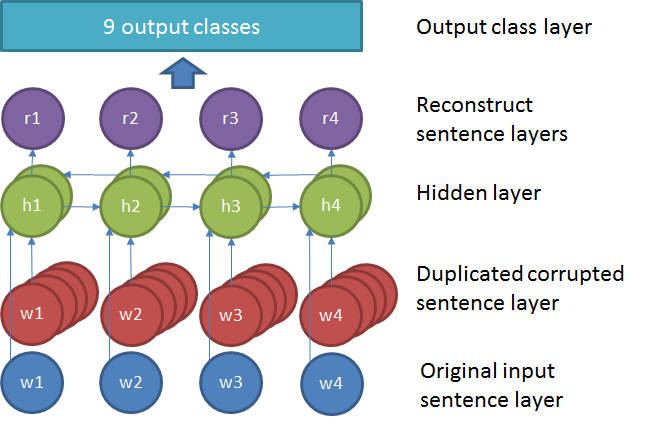
\includegraphics[scale=0.8]{image/overall_archi.png}
  \caption{Overall architecture of the proposed.}
  \label{fig:3}
\end{figure}
Figure~\ref{fig:3} shows the proposed RNN model. 
It consists of four layers: input layers for original inputs and duplicate inputs 
(indicated by red and blue colors), 
hidden layers of either bi-directional or single directional RNN (by green color),
re-constructed sentence layer (by violet color), 
and output layer (by cyan color). 
Word embedding of the original and corrupted sentences is
entered to the input layers. 
The reconstructed sentence layer represents the restored sentence 
from the noisy input. 
The number of units in the hidden layer and reconstructed sentence layer 
is the same as the size of word embedding. 
In the output layer, there are nine unites that corresponds to each 
classification category.
When the model is applied for the prediction, 
we observe the values of the output layer for all time steps,
then choose the category where the highest value is observed.


Both single and bi-directional RNN models are used at the hidden layer.
As for single directional model, LSTM and GRU are used. 
In addition, we also train bi-directional LSTM and GRU with four architectures: 
default, CIFG, peephole and FGR. 
As stated in (Assawinjaipetch et al. 2016) \cite{assawinjaipetch-etal-2016-recurrent}, 
the combination of different RNN architectures in bi-directional model 
such as forward GRU and backward LSTM did not usually improve the model performance.
Therefore, the same architectures are used 
in the bi-directional model in this paper. 
LSTM peephole is expected to achieve the best result due to its 
capability to consider the internal state of the previous time.